\mode*

\section{Behållare}

\subsection{Listor}

\begin{frame}[fragile]
  \lstinline[basicstyle=\huge,mathescape]{var = [ item0, $\dotsc$, itemN ]}
\end{frame}

\begin{frame}[fragile]
  \begin{example}
    \begin{lstlisting}
names = ["Adam", "Bertil", "Cesar"]
print(names[0])
print(names[2])
    \end{lstlisting}
  \end{example}
\end{frame}

\begin{frame}
  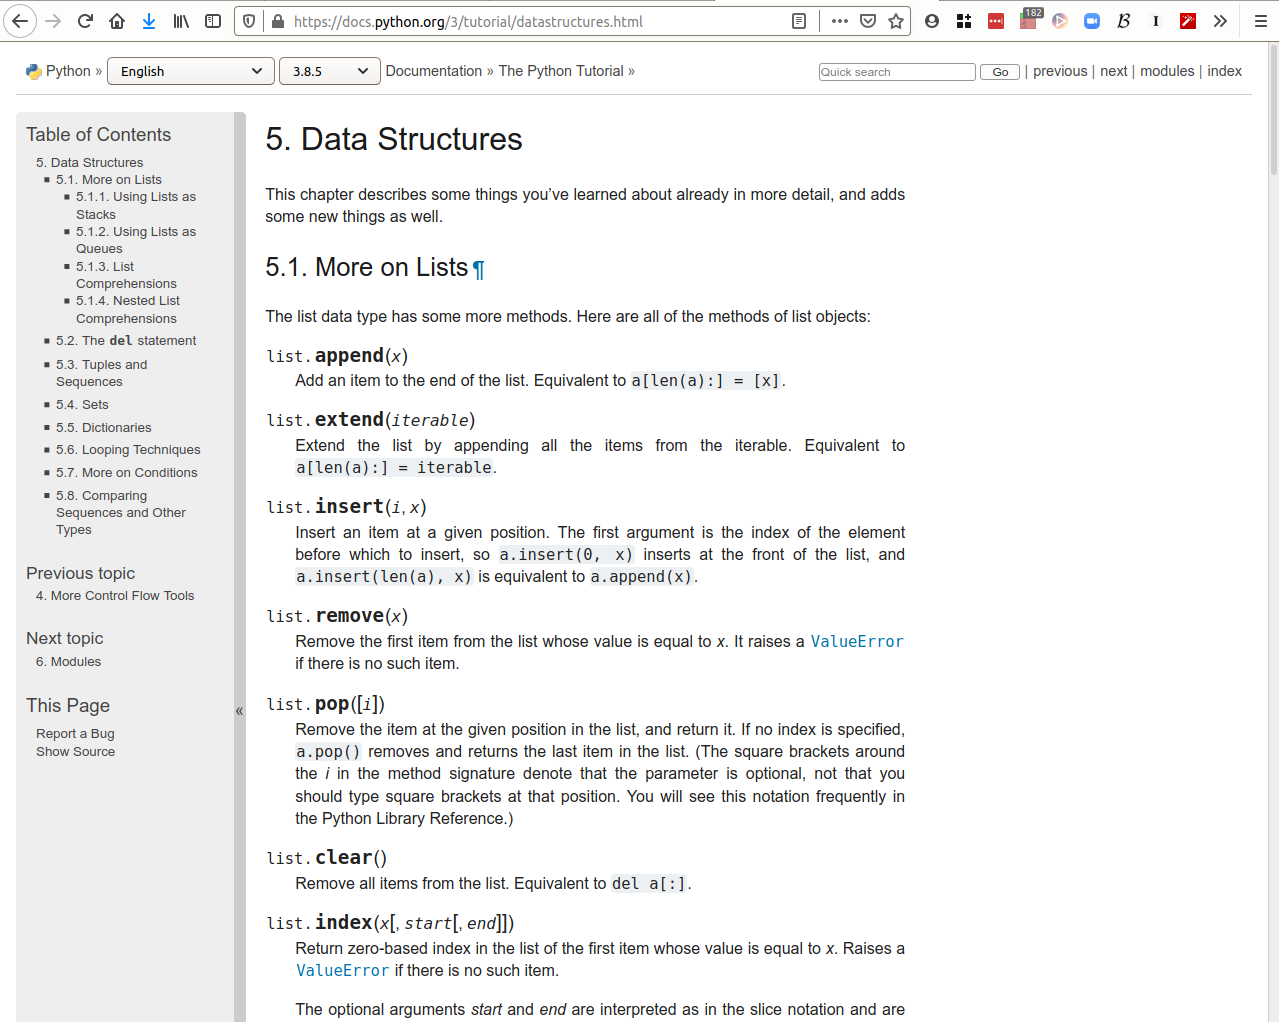
\includegraphics[width=\columnwidth]{figs/docs-lists.png}
\end{frame}

\begin{frame}[fragile]
  \begin{example}[extend\textunderscore{}lists.py]
    \lstinputlisting{examples/extend_lists.py}
  \end{example}
\end{frame}

\begin{frame}[fragile]
  \begin{example}[Aritmetiska \emph{hel}talsföljder]
    \begin{lstlisting}
print(range(10))
print(range(0, 10))
print(range(1, 10, 2))
    \end{lstlisting}
  \end{example}
\end{frame}


\begin{frame}[fragile]
  \lstinline[basicstyle=\huge]{var = [ f(x) for x in lst ]}
\end{frame}

\begin{frame}[fragile]
  \begin{example}[List comprehensions]
    \begin{lstlisting}
squares = [ x**2 for x in range(10) ]
    \end{lstlisting}
  \end{example}
\end{frame}


\subsection{Stackar och köer}

\begin{frame}[fragile]
  \begin{example}[pile.py]
    \lstinputlisting{examples/pile.py}
  \end{example}
\end{frame}

\begin{frame}[fragile]
  \begin{example}[queue.py]
    \lstinputlisting{examples/queue.py}
  \end{example}
\end{frame}

\begin{frame}
  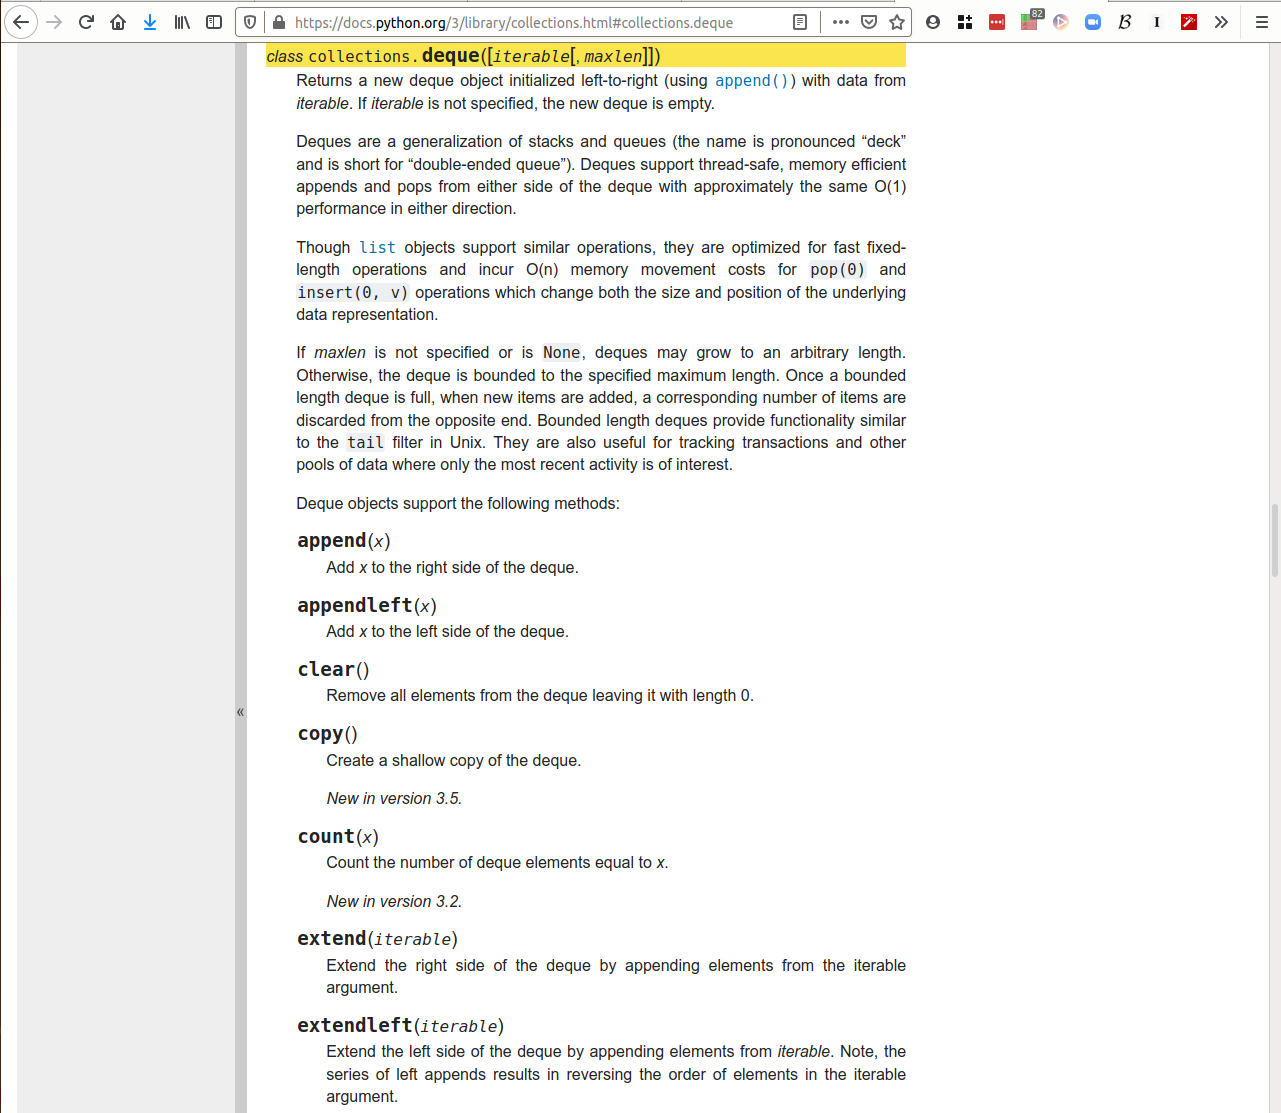
\includegraphics[width=\columnwidth]{figs/docs-deque.png}
\end{frame}


\subsection{Mängder}

\begin{frame}[fragile]
  \begin{example}[sets.py]
    \lstinputlisting{examples/sets.py}
  \end{example}
\end{frame}


\subsection{Uppslagslistor}

\begin{frame}
  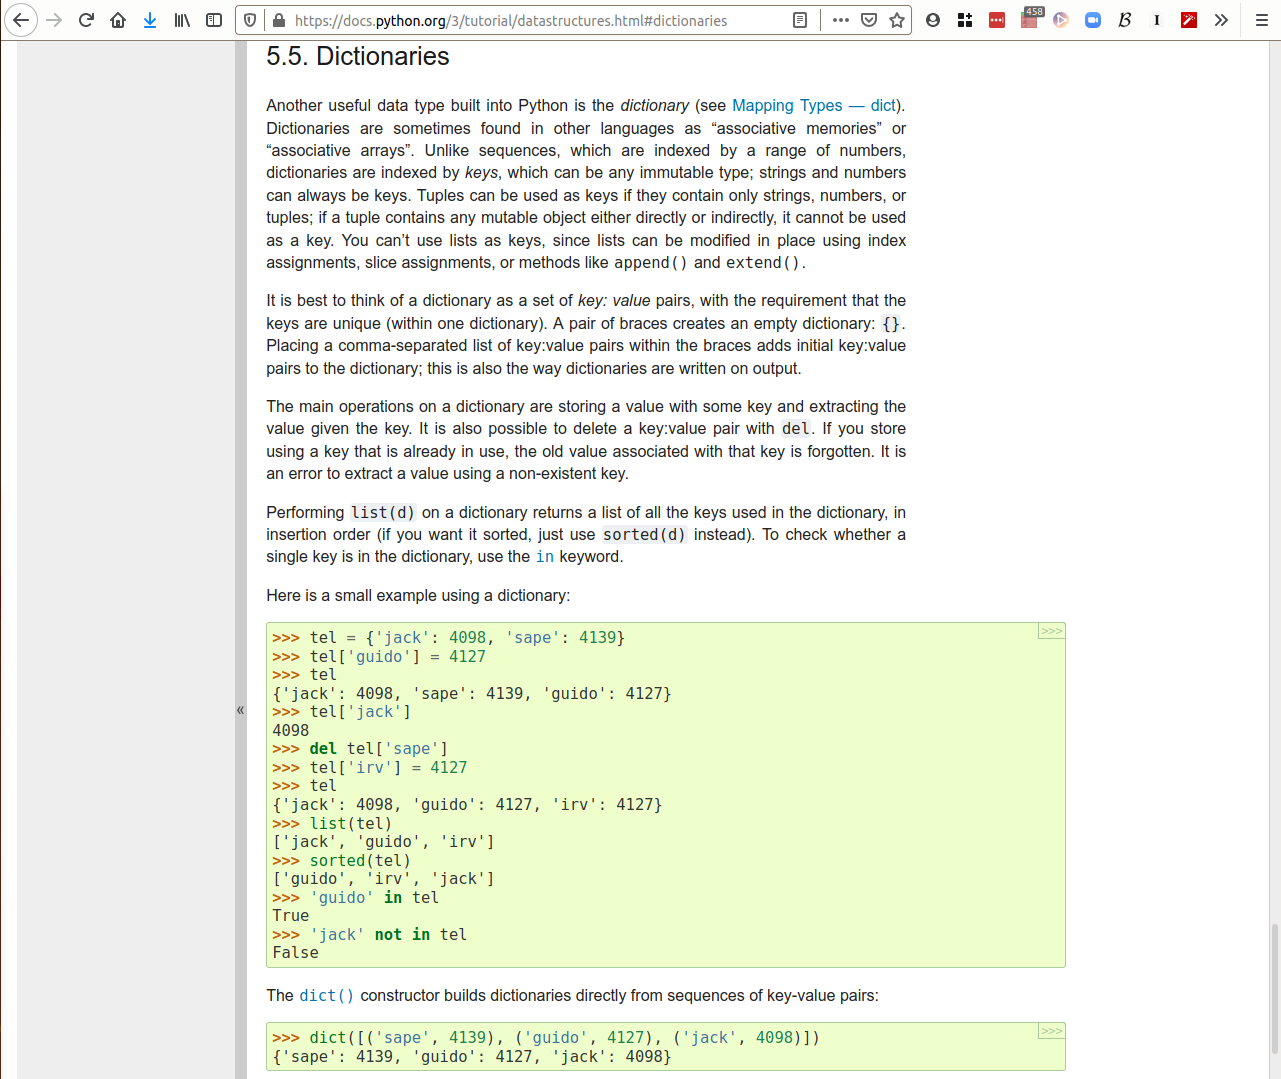
\includegraphics[width=\columnwidth]{figs/docs-dicts.png}
\end{frame}

\begin{frame}[fragile]
  \begin{example}[phone.py]
    \lstinputlisting{examples/phone.py}
  \end{example}
\end{frame}


\section{Iterationer med for-slingor}

\subsection{For-slingan}

\begin{frame}[fragile]
  \begin{lstlisting}[basicstyle=\huge,numbers=none]
for item in container:
  print(item)
  \end{lstlisting}
\end{frame}

\begin{frame}[fragile]
  \begin{example}
    \begin{lstlisting}
for i in range(10):
  print(i)
    \end{lstlisting}
  \end{example}
\end{frame}

\begin{frame}[fragile]
  \begin{example}
    \begin{lstlisting}
for p in ["adam", "bertil", "cesar"]:
    print(p)
    \end{lstlisting}
  \end{example}
\end{frame}

\begin{frame}[fragile]
  \begin{example}[phone-for.py]
    \lstinputlisting[linerange=1-10]{examples/phone-for.py}
  \end{example}
\end{frame}



\subsection{Tuppler}

\begin{frame}[fragile]
  \begin{example}[tuples.py]
    \lstinputlisting{examples/tuples.py}
  \end{example}
\end{frame}


\section{Större exempel}

\subsection{Snygga utskrifter, align\textunderscore{}list.py}

\begin{frame}[fragile]
  \lstinputlisting[linerange=6-13,firstnumber=6]{examples/align_list.py}
\end{frame}

\begin{frame}[fragile]
  \lstinputlisting[linerange=14-25,firstnumber=14]{examples/align_list.py}
\end{frame}


\subsection{Svårare gissningar, guess.py}

\begin{frame}[fragile]
  \lstinputlisting[linerange=5-10,firstnumber=5]{examples/guess.py}
\end{frame}

\begin{frame}[fragile]
  \lstinputlisting[linerange=11-25,firstnumber=11]{examples/guess.py}
\end{frame}

\begin{frame}[fragile]
  \lstinputlisting[linerange=11-13,firstnumber=11]{examples/guess.py}
  \lstinputlisting[firstline=24,firstnumber=24]{examples/guess.py}
\end{frame}

\subsection{Multiplikationskolumner, multcol.py}

\begin{frame}[fragile,allowframebreaks]
  \lstinputlisting[linerange=3-18,firstnumber=3]{examples/multcol.py}
\end{frame}

\begin{frame}[fragile,allowframebreaks]
  \lstinputlisting[firstline=19,firstnumber=19]{examples/multcol.py}
\end{frame}

\subsection{Multiplikationstabell 1--9, multtable.py}

\begin{frame}[fragile,allowframebreaks]
  \lstinputlisting[linerange=3-12,firstnumber=3]{examples/multtable.py}
\end{frame}

\begin{frame}[fragile,allowframebreaks]
  \lstinputlisting[firstline=13,firstnumber=13]{examples/multtable.py}
\end{frame}

\subsection{Multiplikationstabell godtycklig, multtable-expand.py}

\begin{frame}[fragile,allowframebreaks]
  \lstinputlisting[linerange=3-16,firstnumber=3]{examples/multtable-expand.py}
\end{frame}

\begin{frame}[fragile,allowframebreaks]
  \lstinputlisting[firstline=17,firstnumber=17]{examples/multtable-expand.py}
\end{frame}

